%*******10********20********30********40********50********60********70********80
\clearpage

\section{Residual Capabilities after Pure DEF Expansion}

Similar with ASR loading simulation, uni-axial compression test result for DEF expanded concrete model is summarised.

DEF loading simulation results of intensified center 50x50x50mm (labeled as I50), 75x75x75mm (labeled as I75) and uniformly expansion for all part (intensified center 100x100x100mm, labeled as I100), with aggregate percentage of 30\%, are presented.  Alternated case for I50 with 15\% coarse aggregate is also presented.

\begin{figure}[!ht]
\centering
    %*******
    \begin{subfigure}{.33\textwidth}
      \centering
      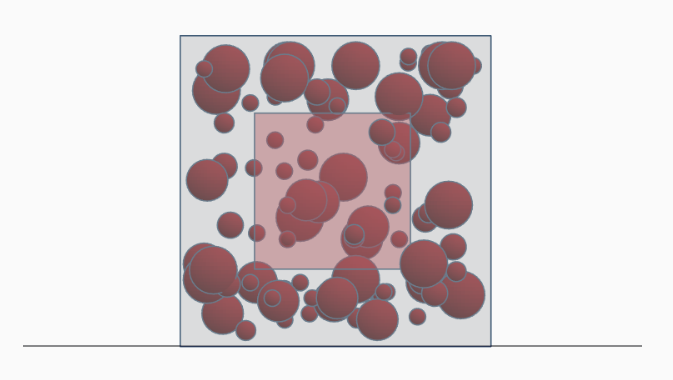
\includegraphics[width=.8\linewidth]{Files/DEF_X/X0_3ds.png}
      \caption{Intensified 50x50x50mm Case\\ I50}
    \end{subfigure}%
    %*******
    \begin{subfigure}{.33\textwidth}
      \centering
      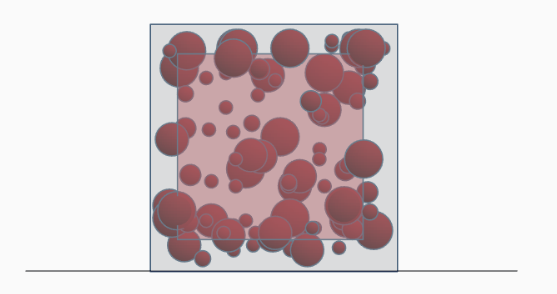
\includegraphics[width=.8\linewidth]{Files/DEF_X/X-5_3ds.png}
      \caption{Intensified 75x75x75mm Case \\ I75}
    \end{subfigure}%
    %*******
    \begin{subfigure}{.33\textwidth}
      \centering
      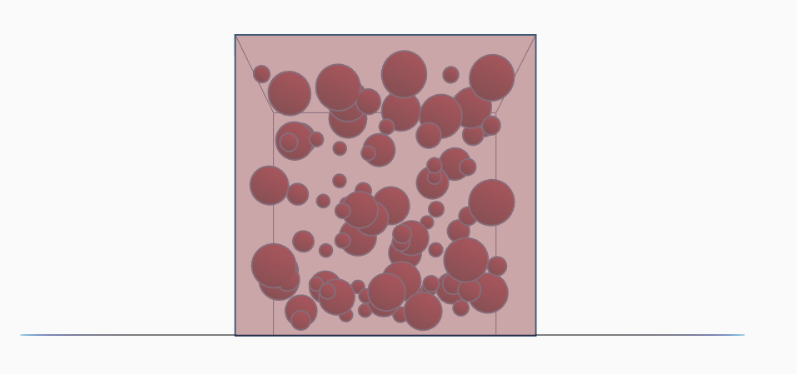
\includegraphics[width=.9\linewidth]{Files/DEF_X/X-1_3ds.png}
      \caption{Intensified 100x100x100mm Case\\ I100}
    \end{subfigure}
    %*******
  \caption{DEF intensified part range}
\end{figure}

\begin{figure}[!h]
\centering
\begin{subfigure}{.5\textwidth}
  \centering
  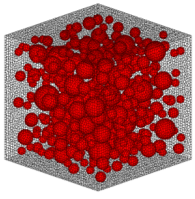
\includegraphics[width=.4\linewidth]{Files/Aggregate/A15.png}
  \caption{15\% Coarse Aggregate}
  \label{fig:A15_model}
\end{subfigure}%
\begin{subfigure}{.5\textwidth}
  \centering
  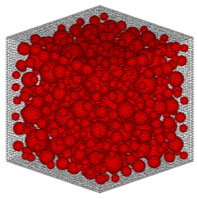
\includegraphics[width=.4\linewidth]{Files/Aggregate/A30.png}
  \caption{30\% Coarse Aggregate}
  \label{fig:A15_model}
\end{subfigure}
\caption{Coarse Aggregate Percentage}
\end{figure}

From Figure \ref{fig:A30X0FIX_LD}, Figure \ref{fig:A30X-5FIX_LD}, Figure \ref{fig:A30X-5FIX_LD} and Figure \ref{fig:A15X0FIX_LD}, Load-Displacement relationships in fix boundary condition uni-axial compression test are shown.

%A30X0FIX

\begin{figure}[ht!]
\centering
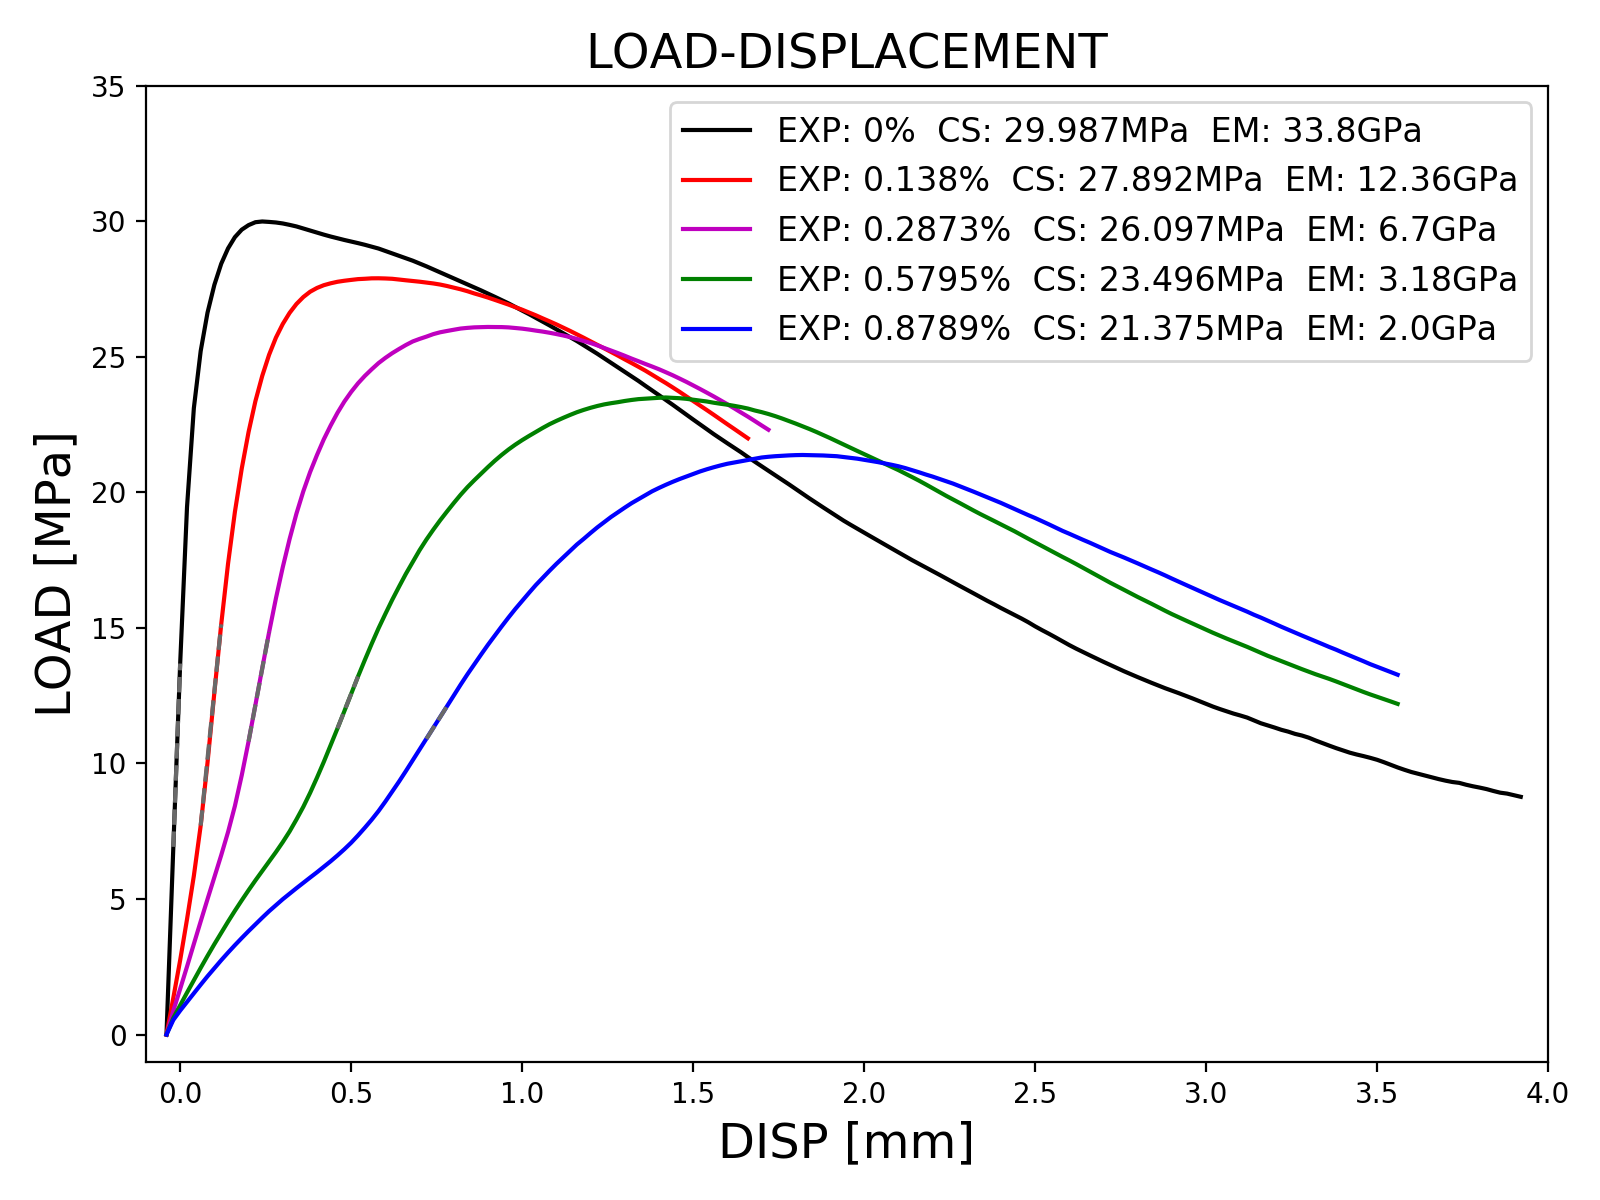
\includegraphics[width=.8\linewidth]{Files/exp_3D/DEF/S13A30FIXX0-LOAD-DISPLACEMENT.png}
  \caption{A30 I50 Fix Load-Displacement}
  \label{fig:A30X0FIX_LD}
\end{figure}

%A30X-5FIX

\begin{figure}[ht!]
\centering
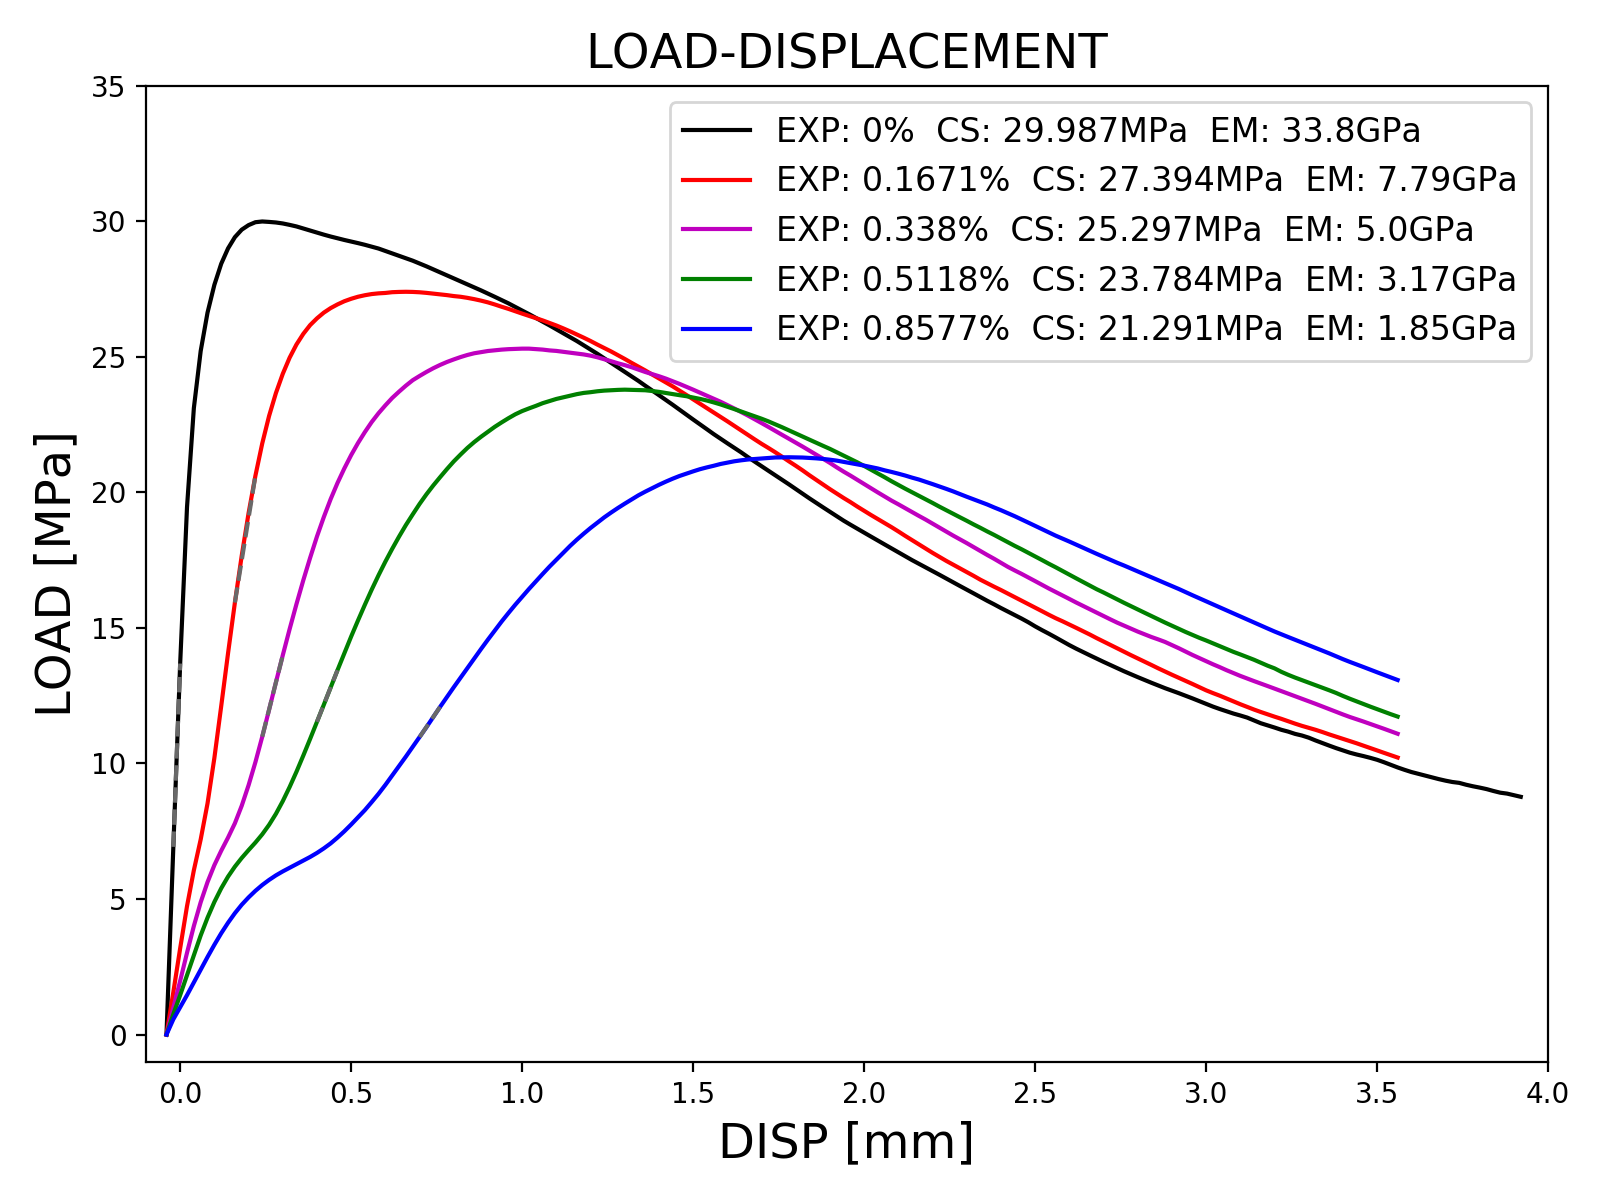
\includegraphics[width=.8\linewidth]{Files/exp_3D/DEF/S13A30FIXX-5-LOAD-DISPLACEMENT.png}
  \caption{A30 I75 Fix Load-Displacement}
  \label{fig:A30X-5FIX_LD}
\end{figure}

%A30X-1FIX

\begin{figure}[ht!]
\centering
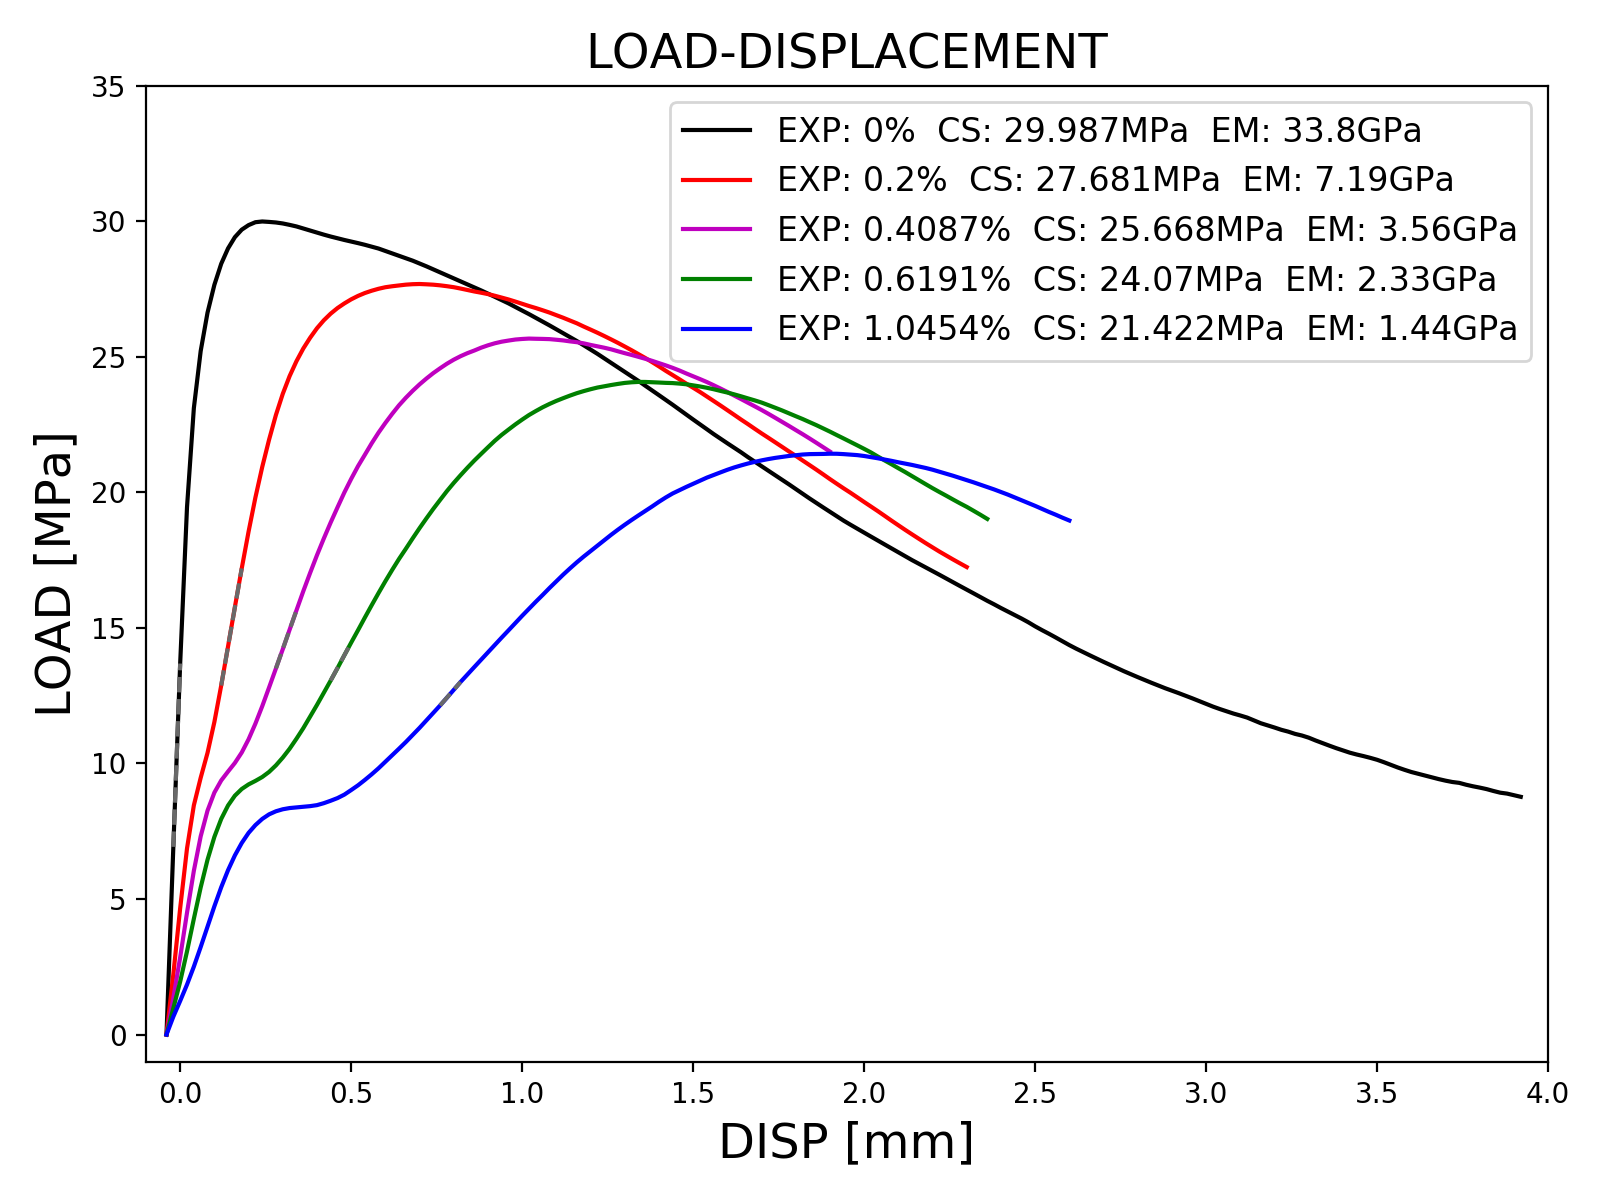
\includegraphics[width=.8\linewidth]{Files/exp_3D/DEF/S13A30FIXX-1-LOAD-DISPLACEMENT.png}
  \caption{A15 I50 Fix Load-Displacement}
  \label{fig:A30X-1FIX_LD}
\end{figure}

%A15X0FIX

\begin{figure}[ht!]
\centering
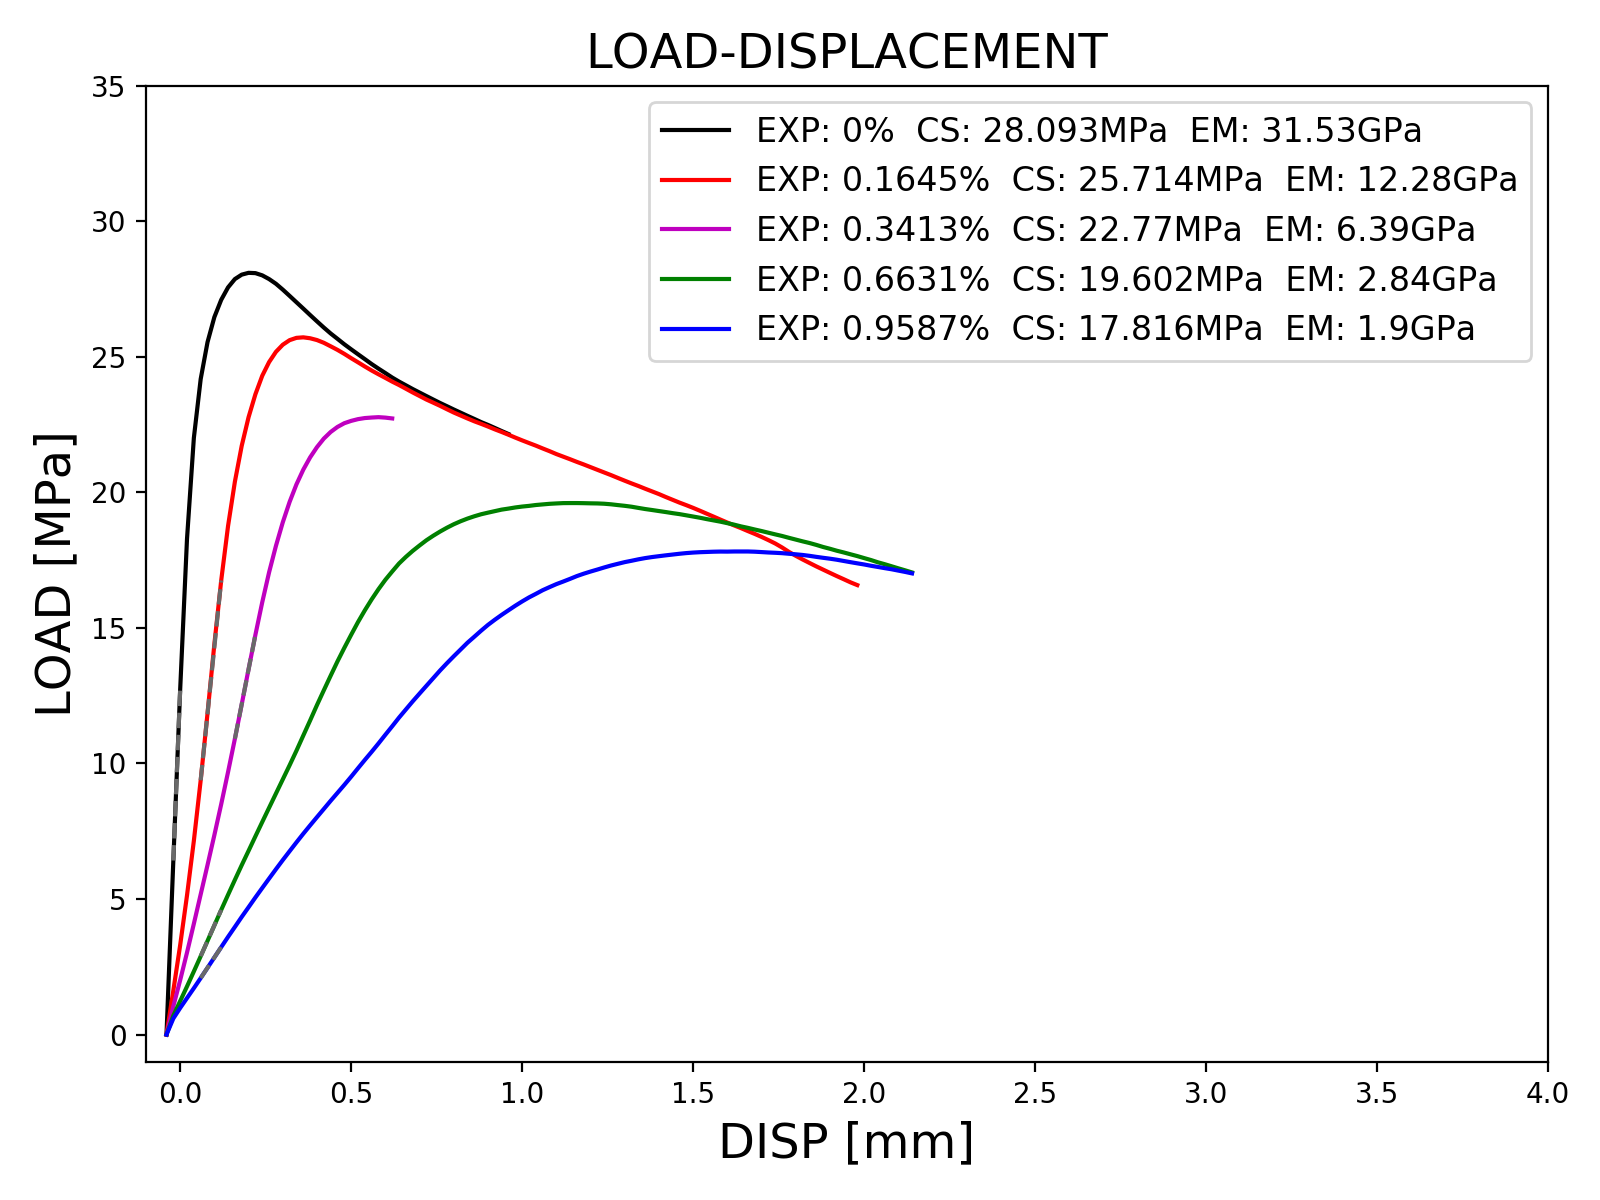
\includegraphics[width=.8\linewidth]{Files/exp_3D/DEF/S13A15FIXX0-LOAD-DISPLACEMENT.png}
  \caption{A15 I50 Fix Load-Displacement}
  \label{fig:A15X0FIX_LD}
\end{figure}

\clearpage

The simulation result in residual compressive strength of DEF damaged models here is plotted, as in Figure \ref{DEF_CS_summary}, which can be seen that different with ASR simulation, the decresaing trend in compressive strength is not significantly influenced by factors such as percentage of coarse aggregate, especially the intensified zone range of DEF expansion.

However, same as in ASR expansion elastic modulus simulation results, the residual elasic modulus in all DEF cases are also significantly lower than expanerimental results. Adjustment in mechnical properties of DEF expanded concrete model may also require modification in further research.

\begin{figure}[ht!]
\centering
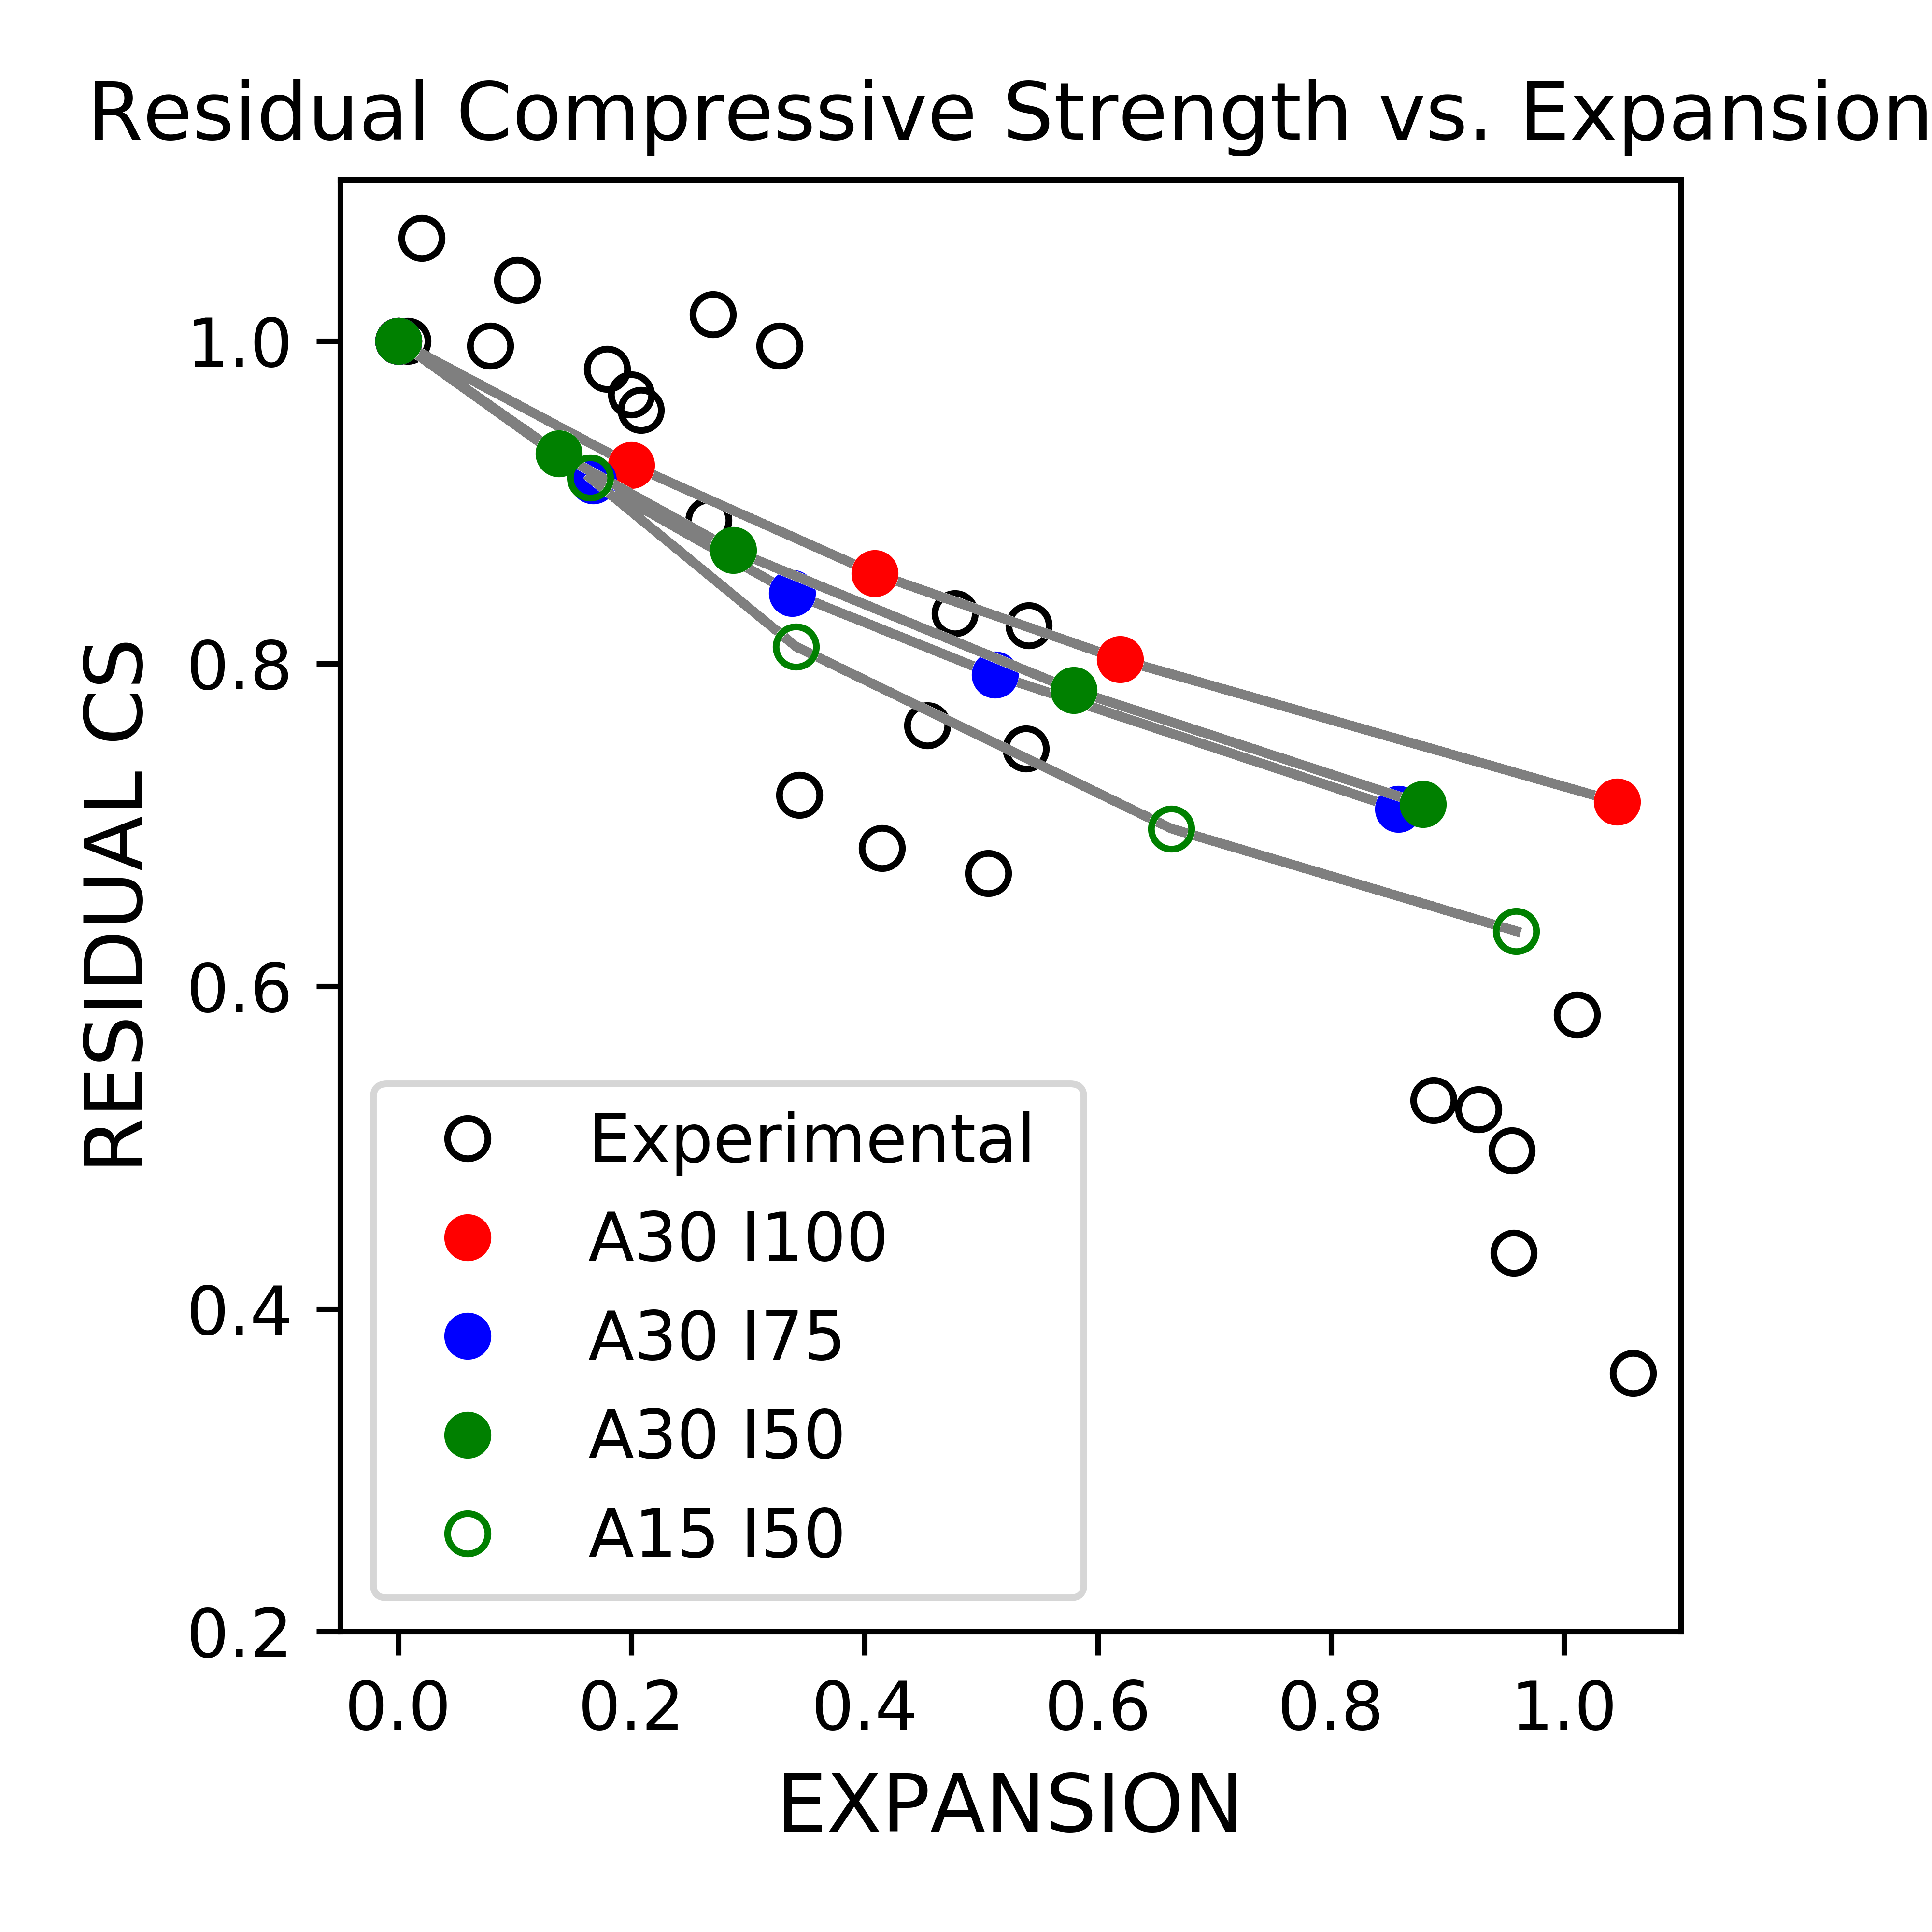
\includegraphics[width=.8\linewidth]{Files/CS_plot/DEFCS_all.png}
  \caption{DEF Compressive Strength Comparing With Experimental Results}
  \label{DEF_CS_summary}
\end{figure}

\begin{figure}[ht!]
\centering
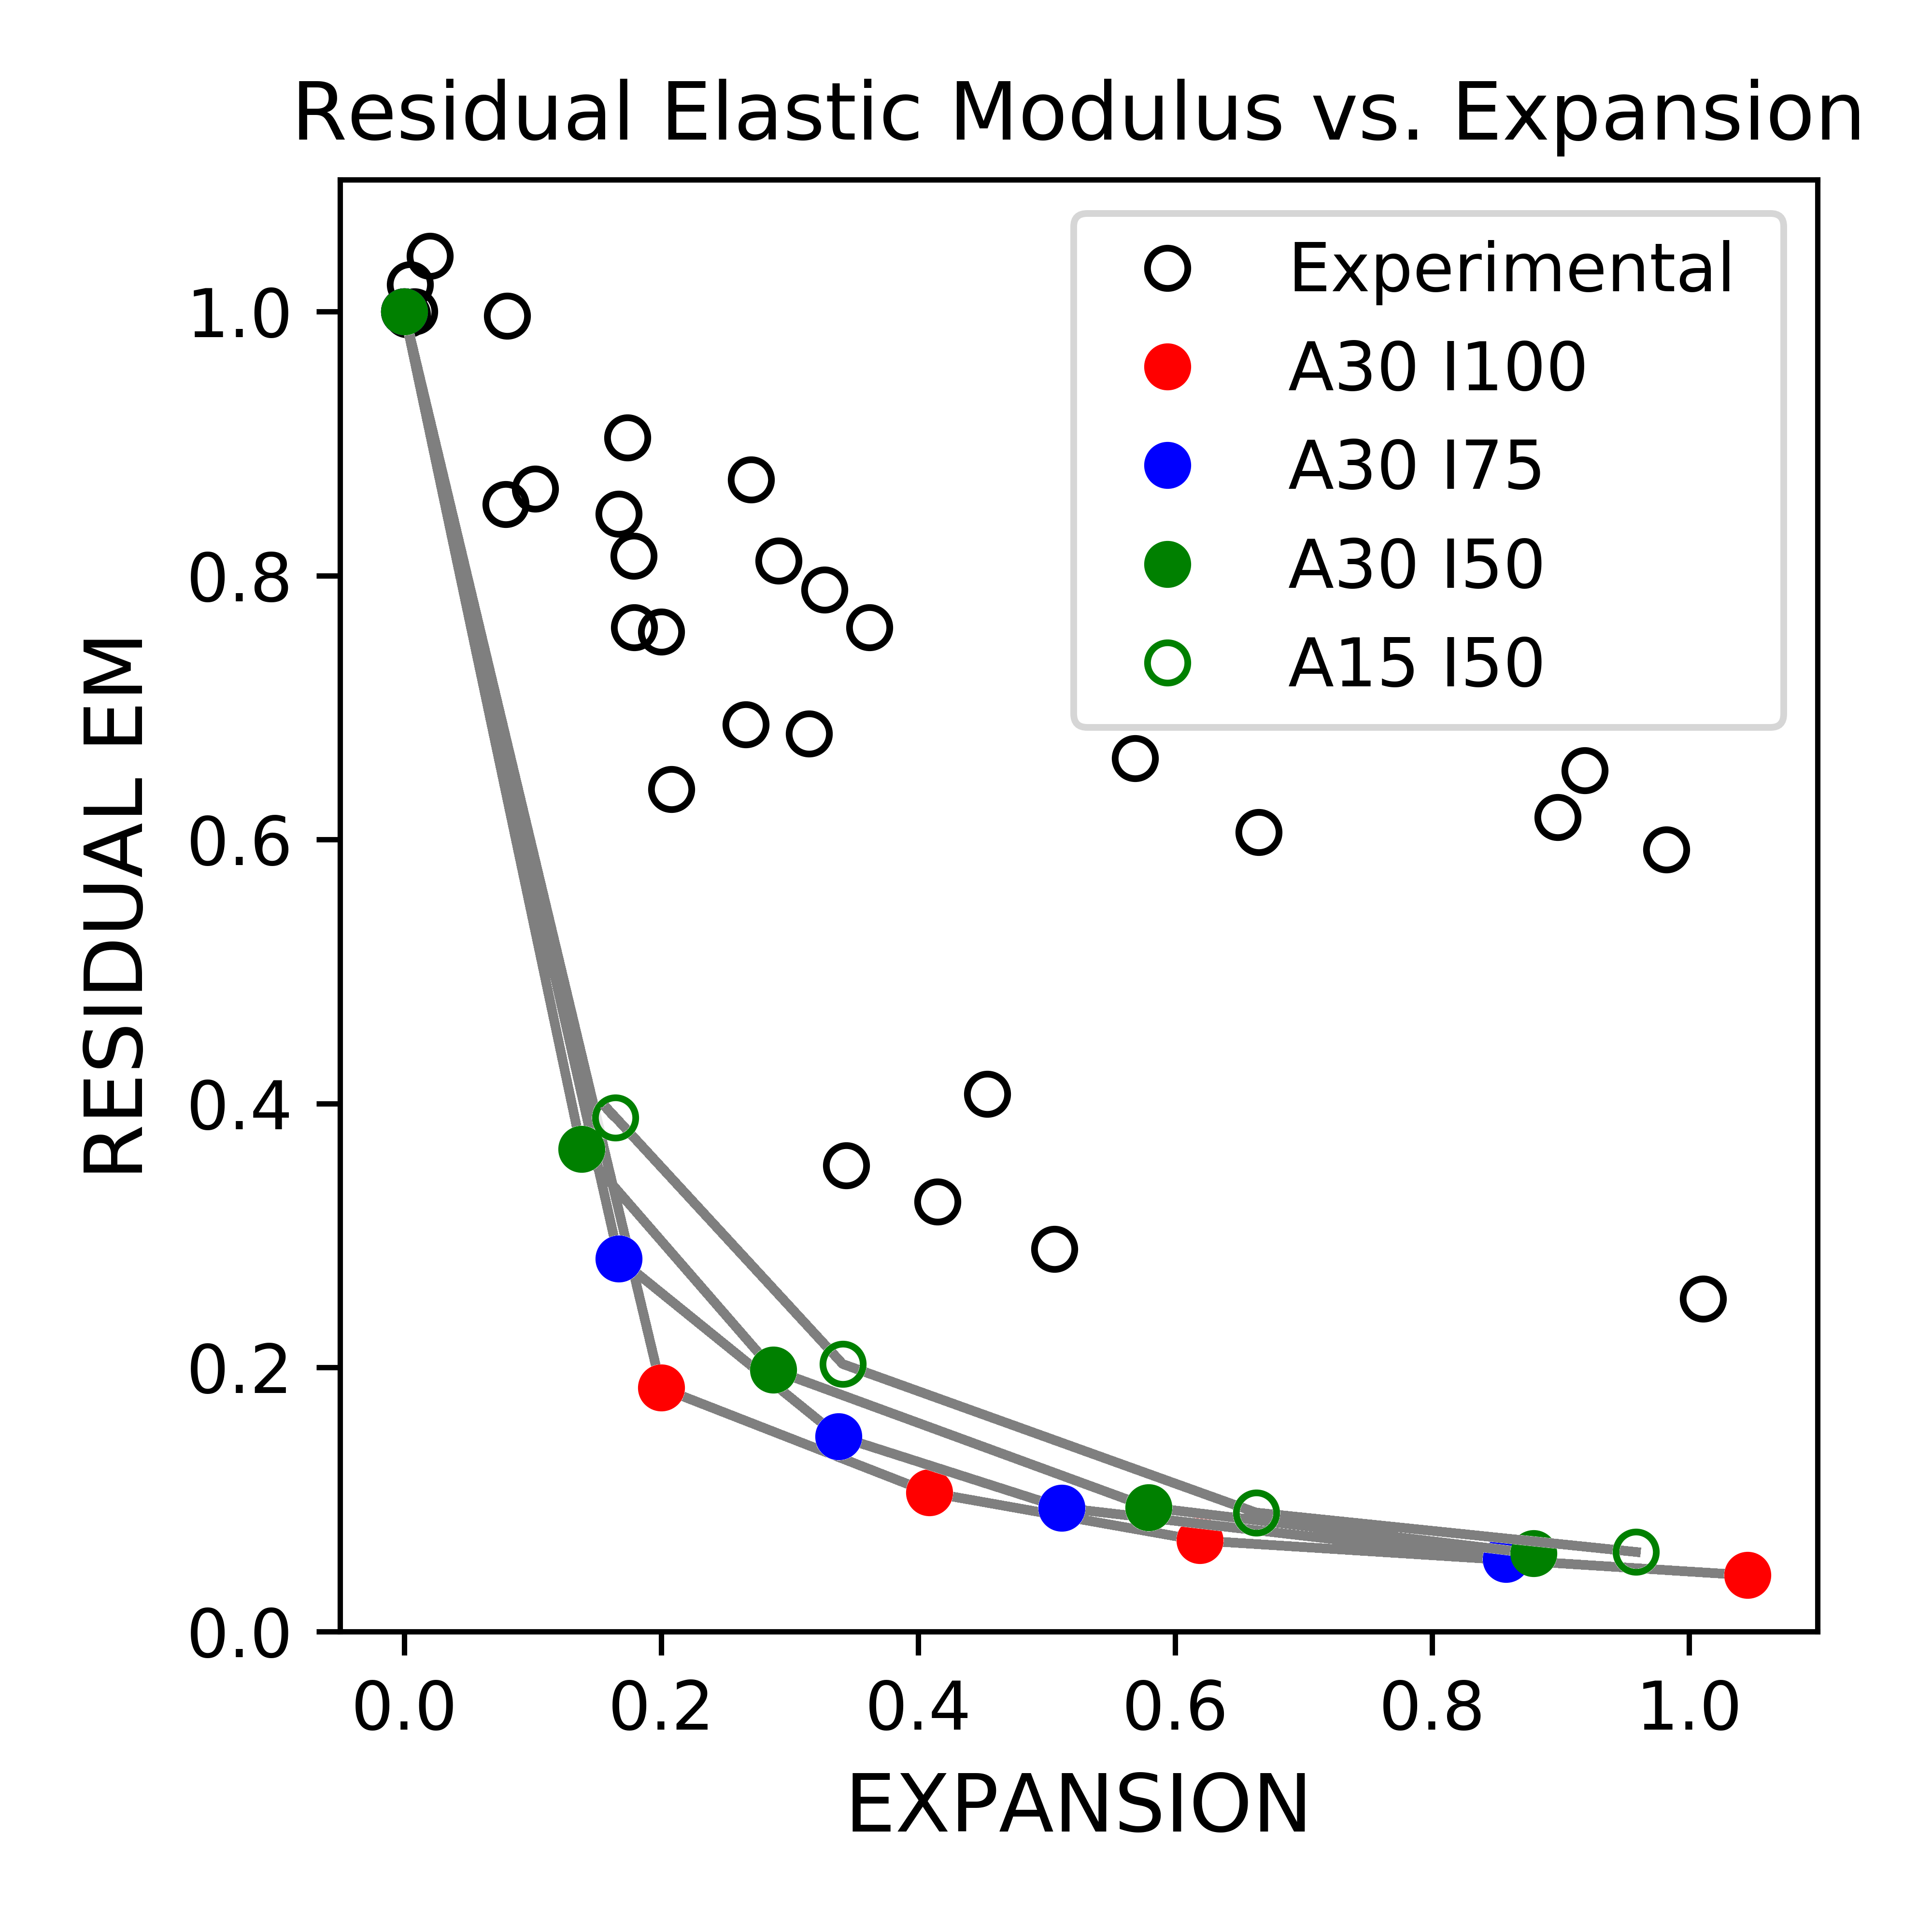
\includegraphics[width=.8\linewidth]{Files/CS_plot/DEFEM_all.png}
  \caption{DEF Elastic Modulus Comparing With Experimental Results}
  \label{DEF_EM_summary}
\end{figure}


In general, the trend in residual compressive strength changing obtained from simulation is not far from the results collected from previous experimental results. With the increasing of global expansion in one-dimensional, compressive strength gradually decrease in all cases.

In some of the Load-Displacement plotting, discontinuity in Elastic Modulus is shown in the loading result, especially in A30 I75 cases and A15 I50 cases. This phenomena is also very common in damaged concrete in reality as the Elastic Modulus would change when cracks are closed horizontally.

As shown in Figure \ref{DEFA30vsA15}, if comparing 30\% coarse aggregate results(with center 50x50x50mm zone given intensified DEF expansion), which are labeled as A30 I50, and 15\% coarse aggregate results(with center 50x50x50mm zone given intensified DEF expansion), which are labeled as A15 I50, it can be seen that the residual compressive strength in 15\% coarse aggregate cases are relative lower than the 30\% coarse aggregate cases. However, if compare the residual elastic modulus of A30 I50 and A15 I50 in Figure \ref{DEF_EM_summary}, in this time, residual compressive strength in 15\% coarse aggregate cases are relative higher than the 30\% coarse aggregate cases.

\begin{figure}[ht!]
\centering
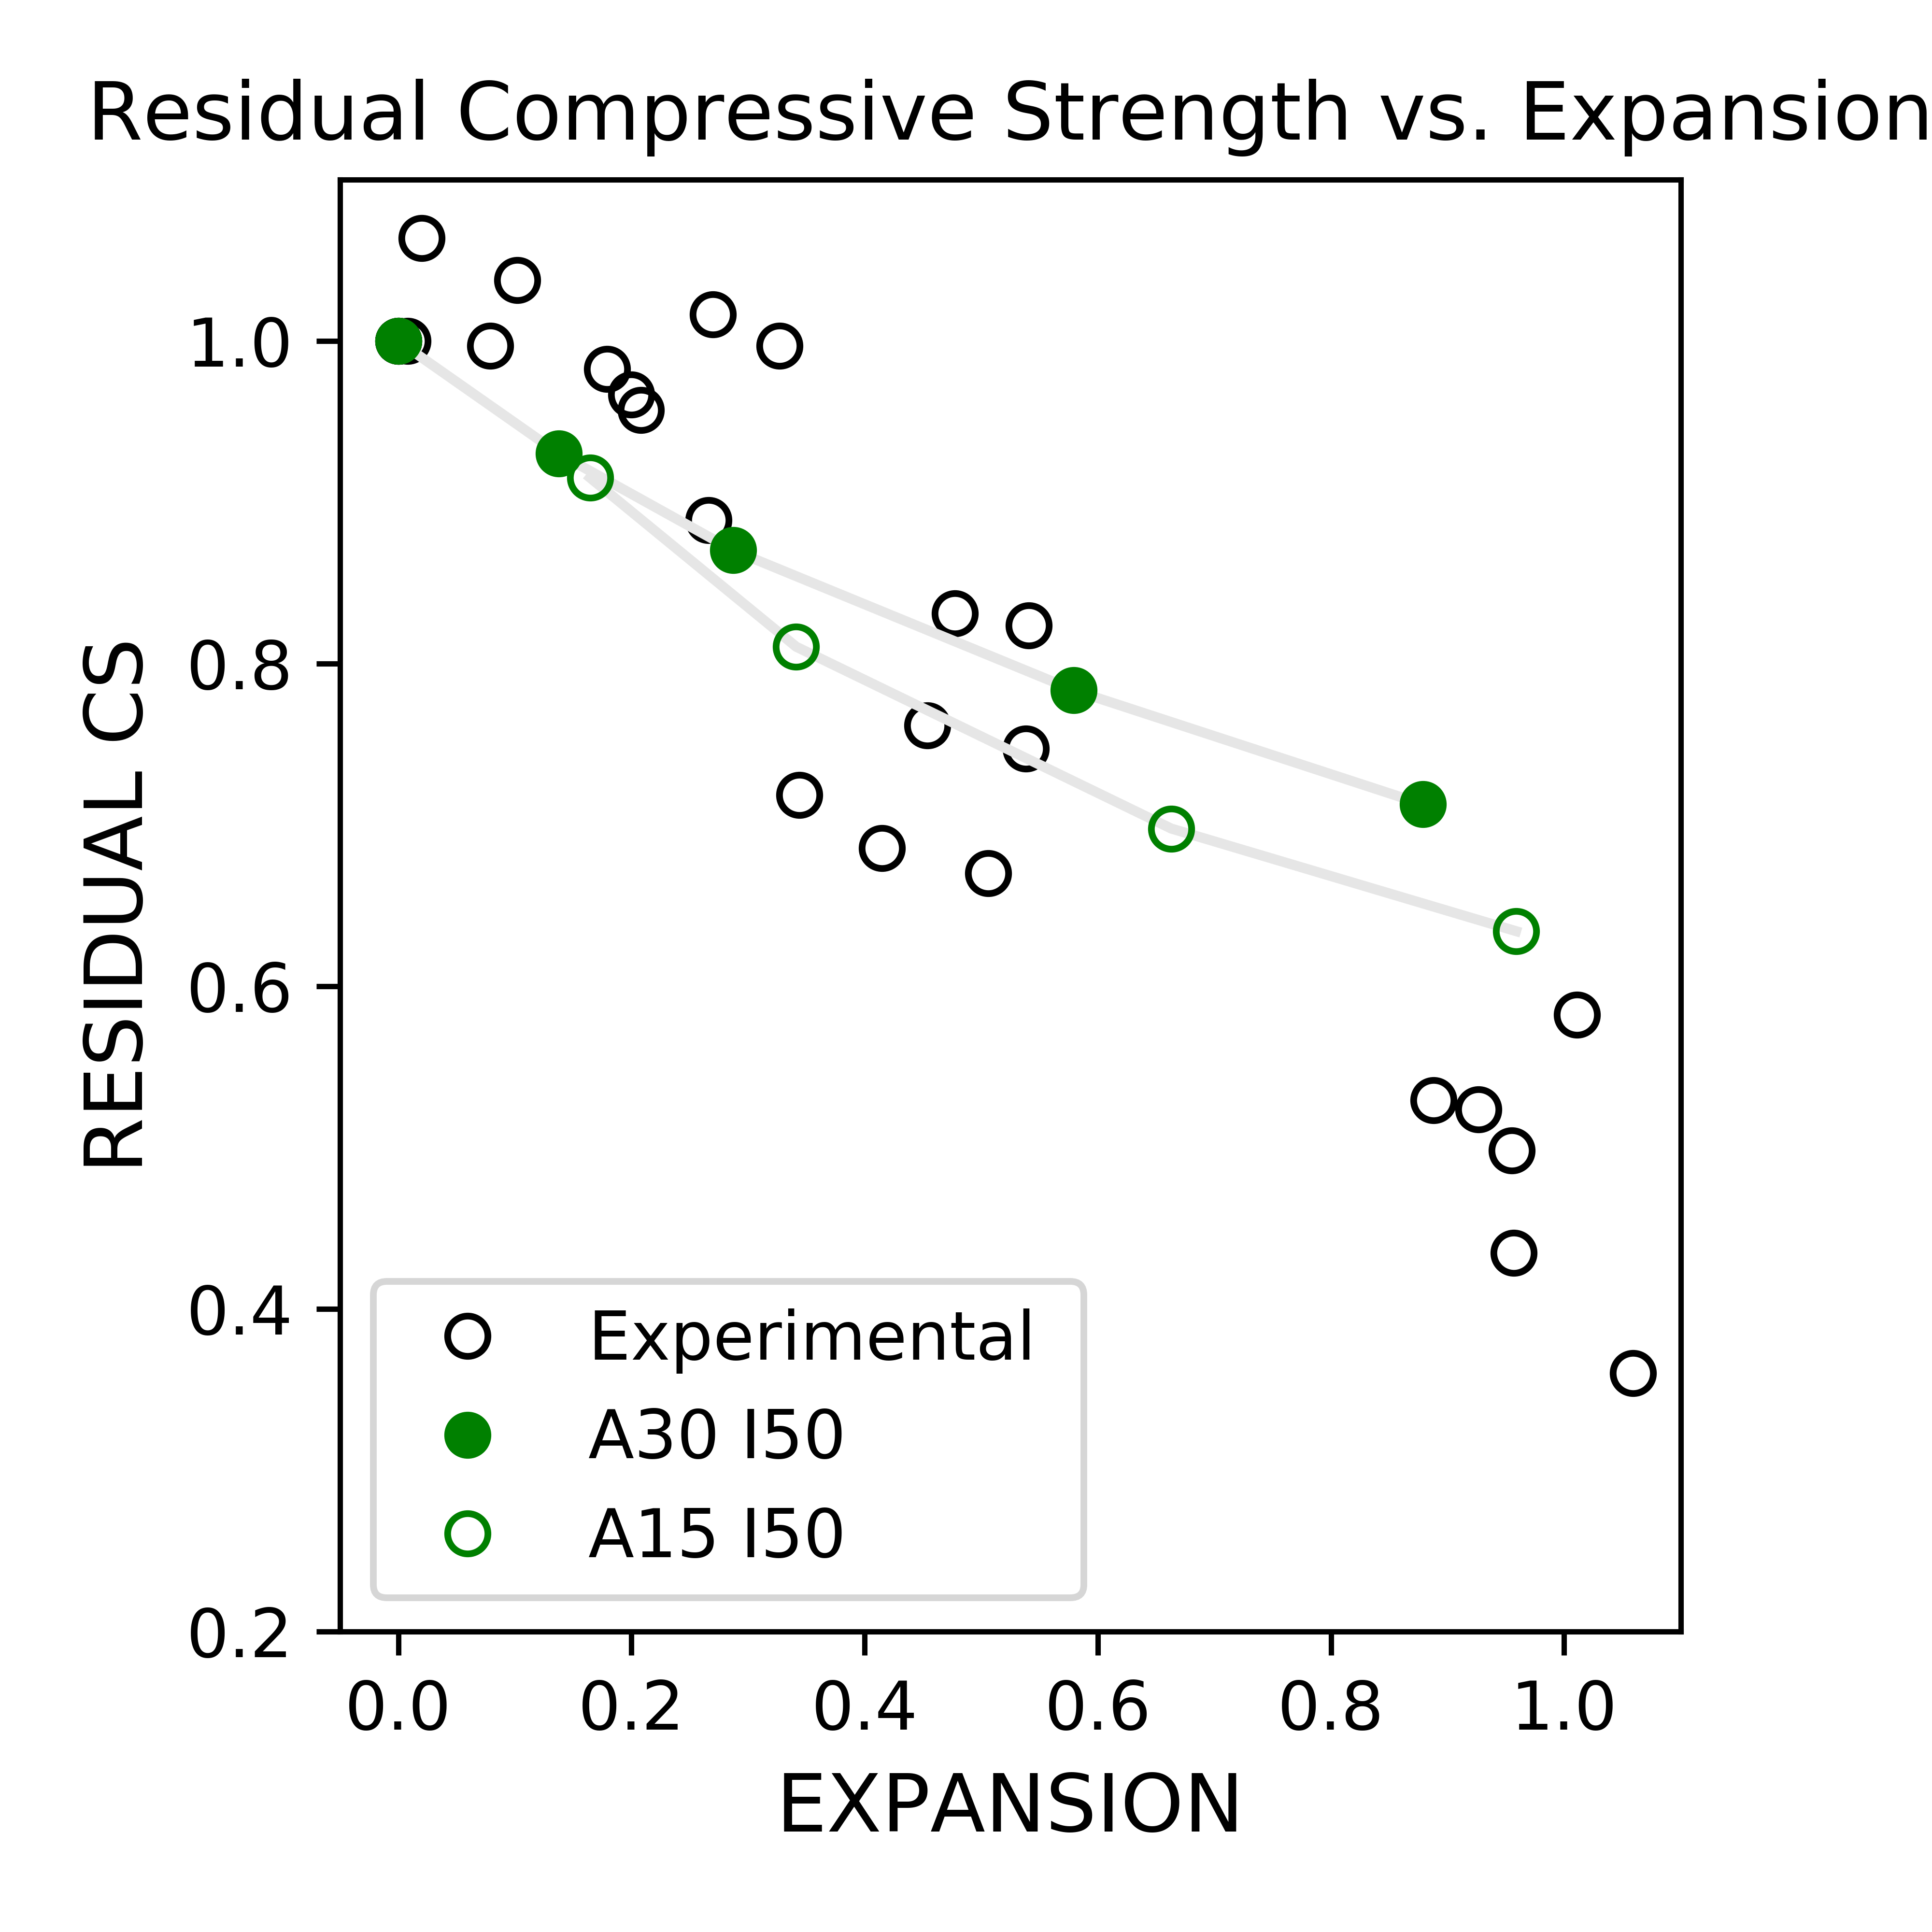
\includegraphics[width=.8\linewidth]{Files/CS_plot/DEFCS2.png}
  \caption{DEF Compressive Strength Comparing With Experimental Results}
  \label{DEFA30vsA15}
\end{figure}

However, the residual compressive strength results for same 30\% coarse aggregate models with different DEF intensified zone range are very close. A30 I100 case, as given overall uniform DEF expansion, shows slightly advantage in residual compressive strength comparing to other 2 cases with non-uniformed expansion, but this difference is only around 8\%.

\begin{figure}[ht!]
\centering
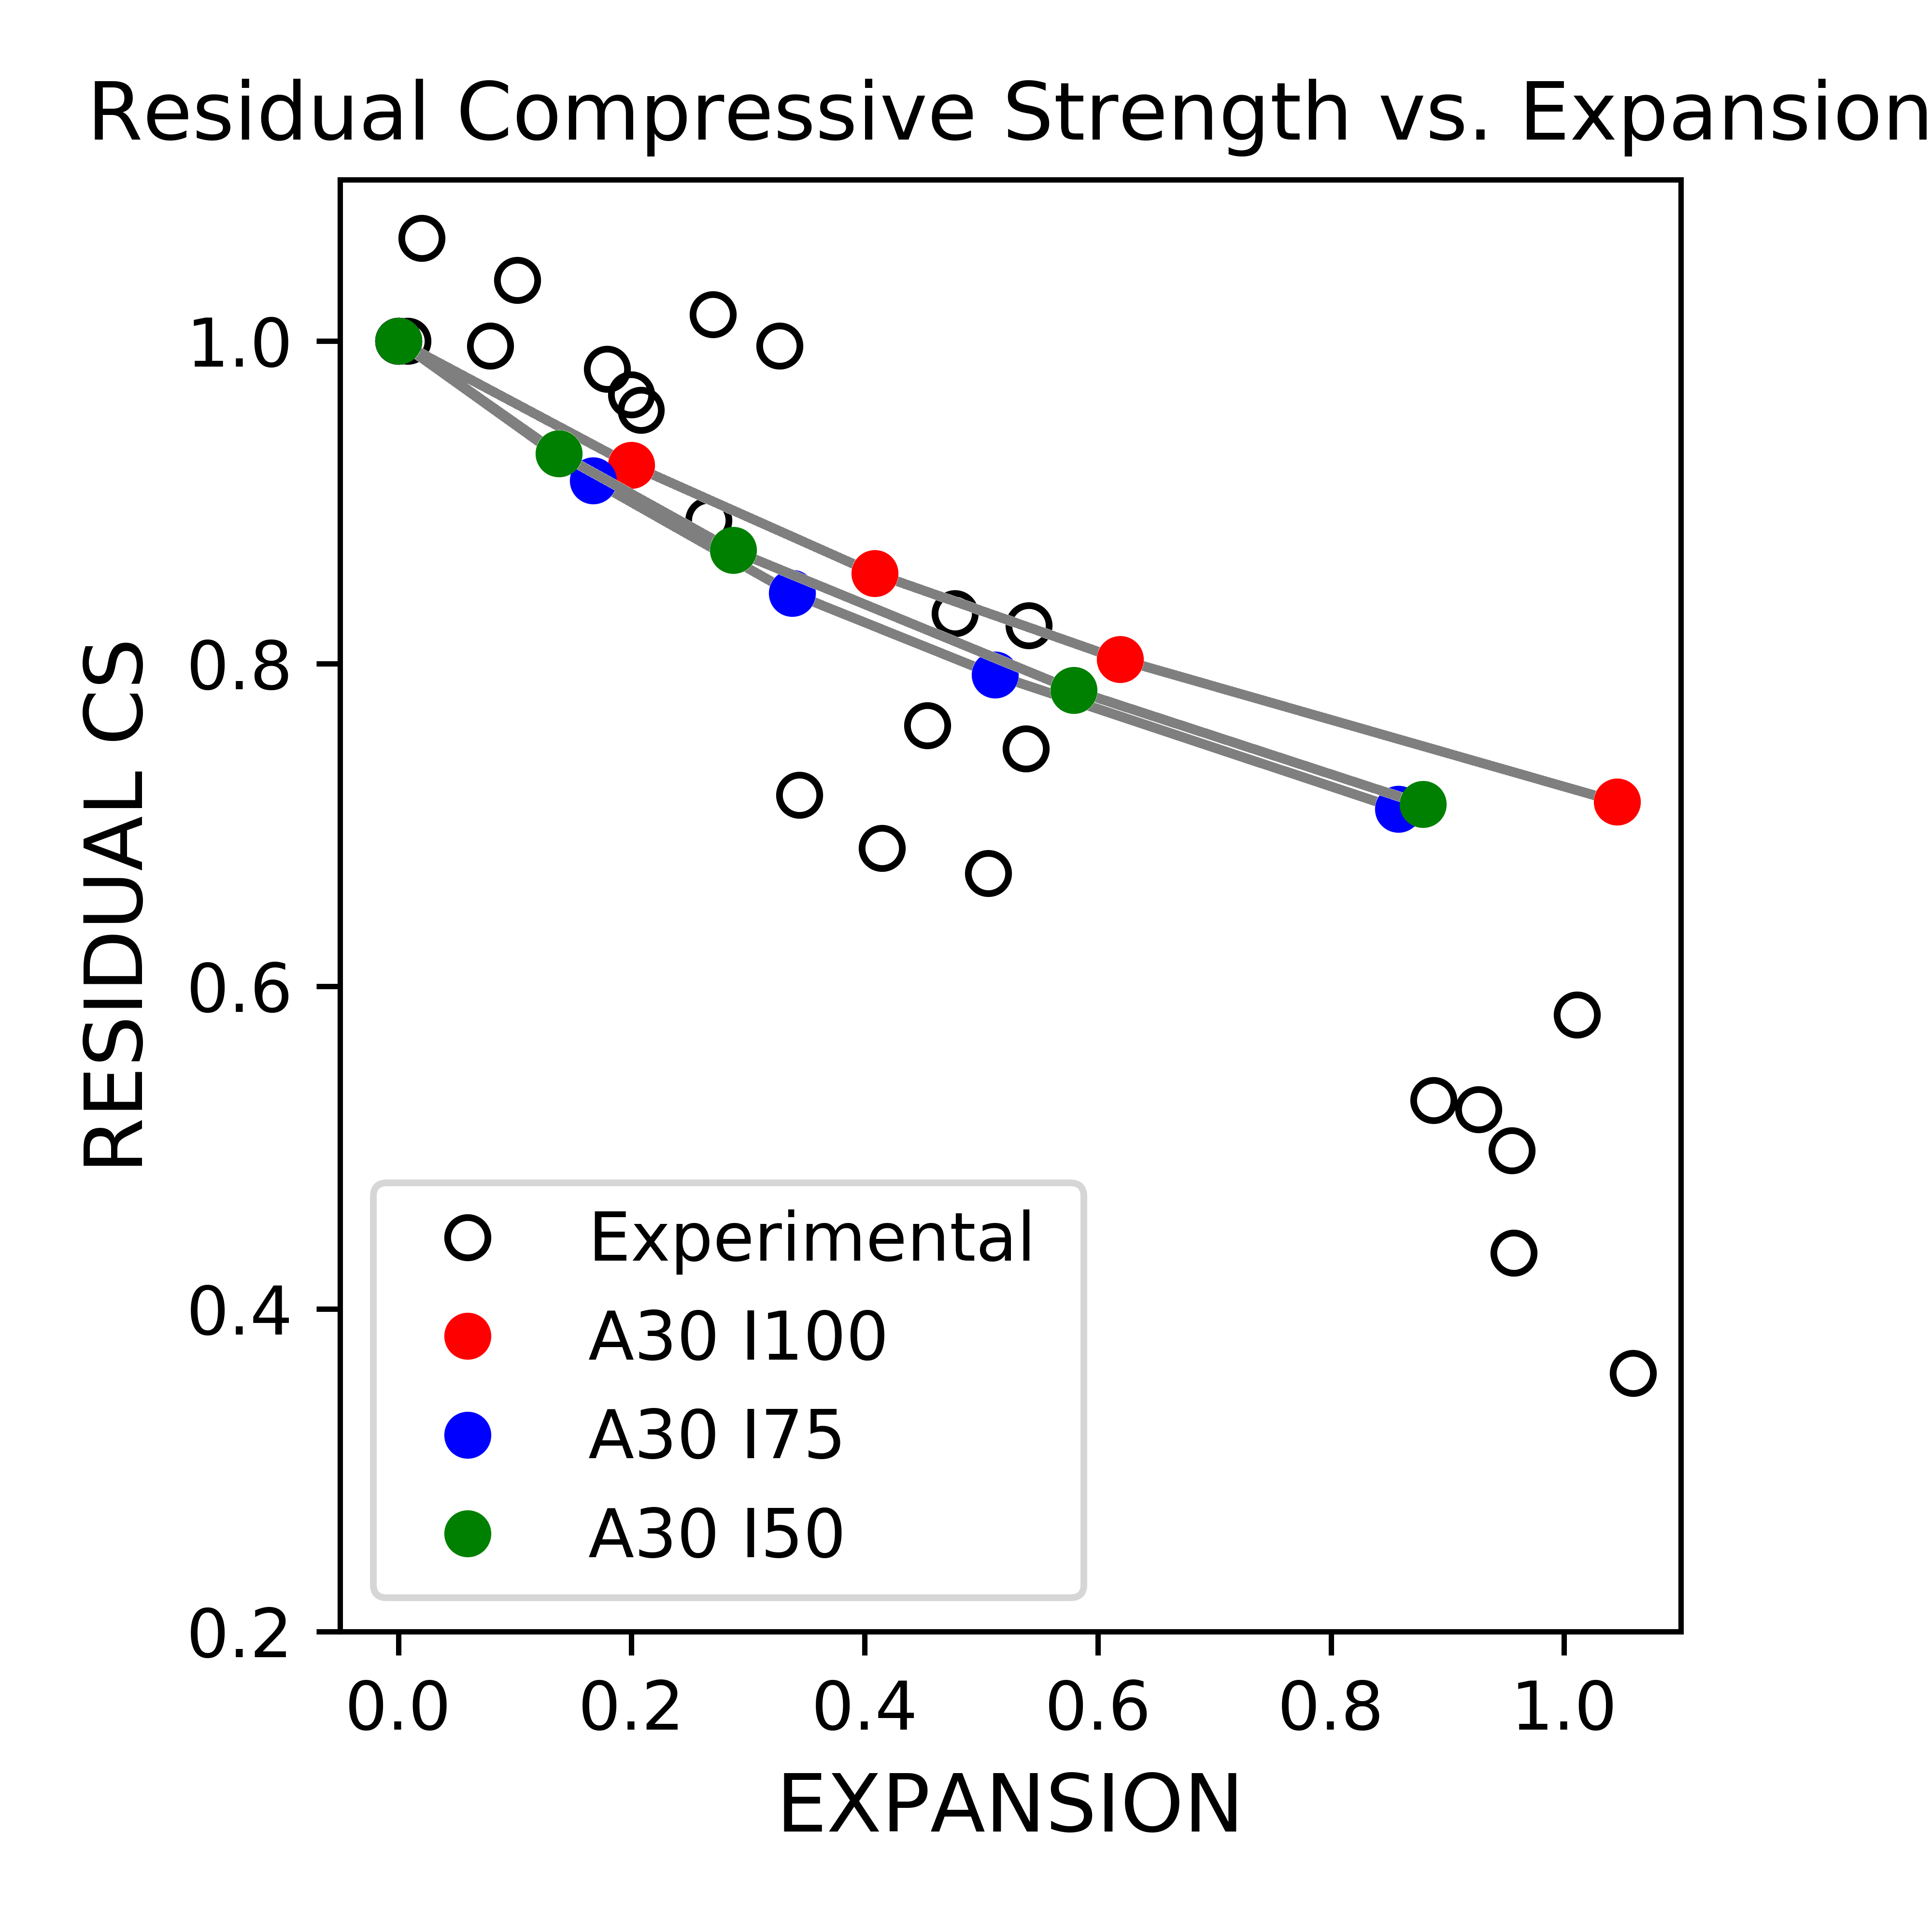
\includegraphics[width=.8\linewidth]{Files/CS_plot/DEFCS3.png}
  \caption{DEF Compressive Strength Comparing With Experimental Results}
  \label{DEF_X}
\end{figure}

\begin{figure}[ht!]
\centering
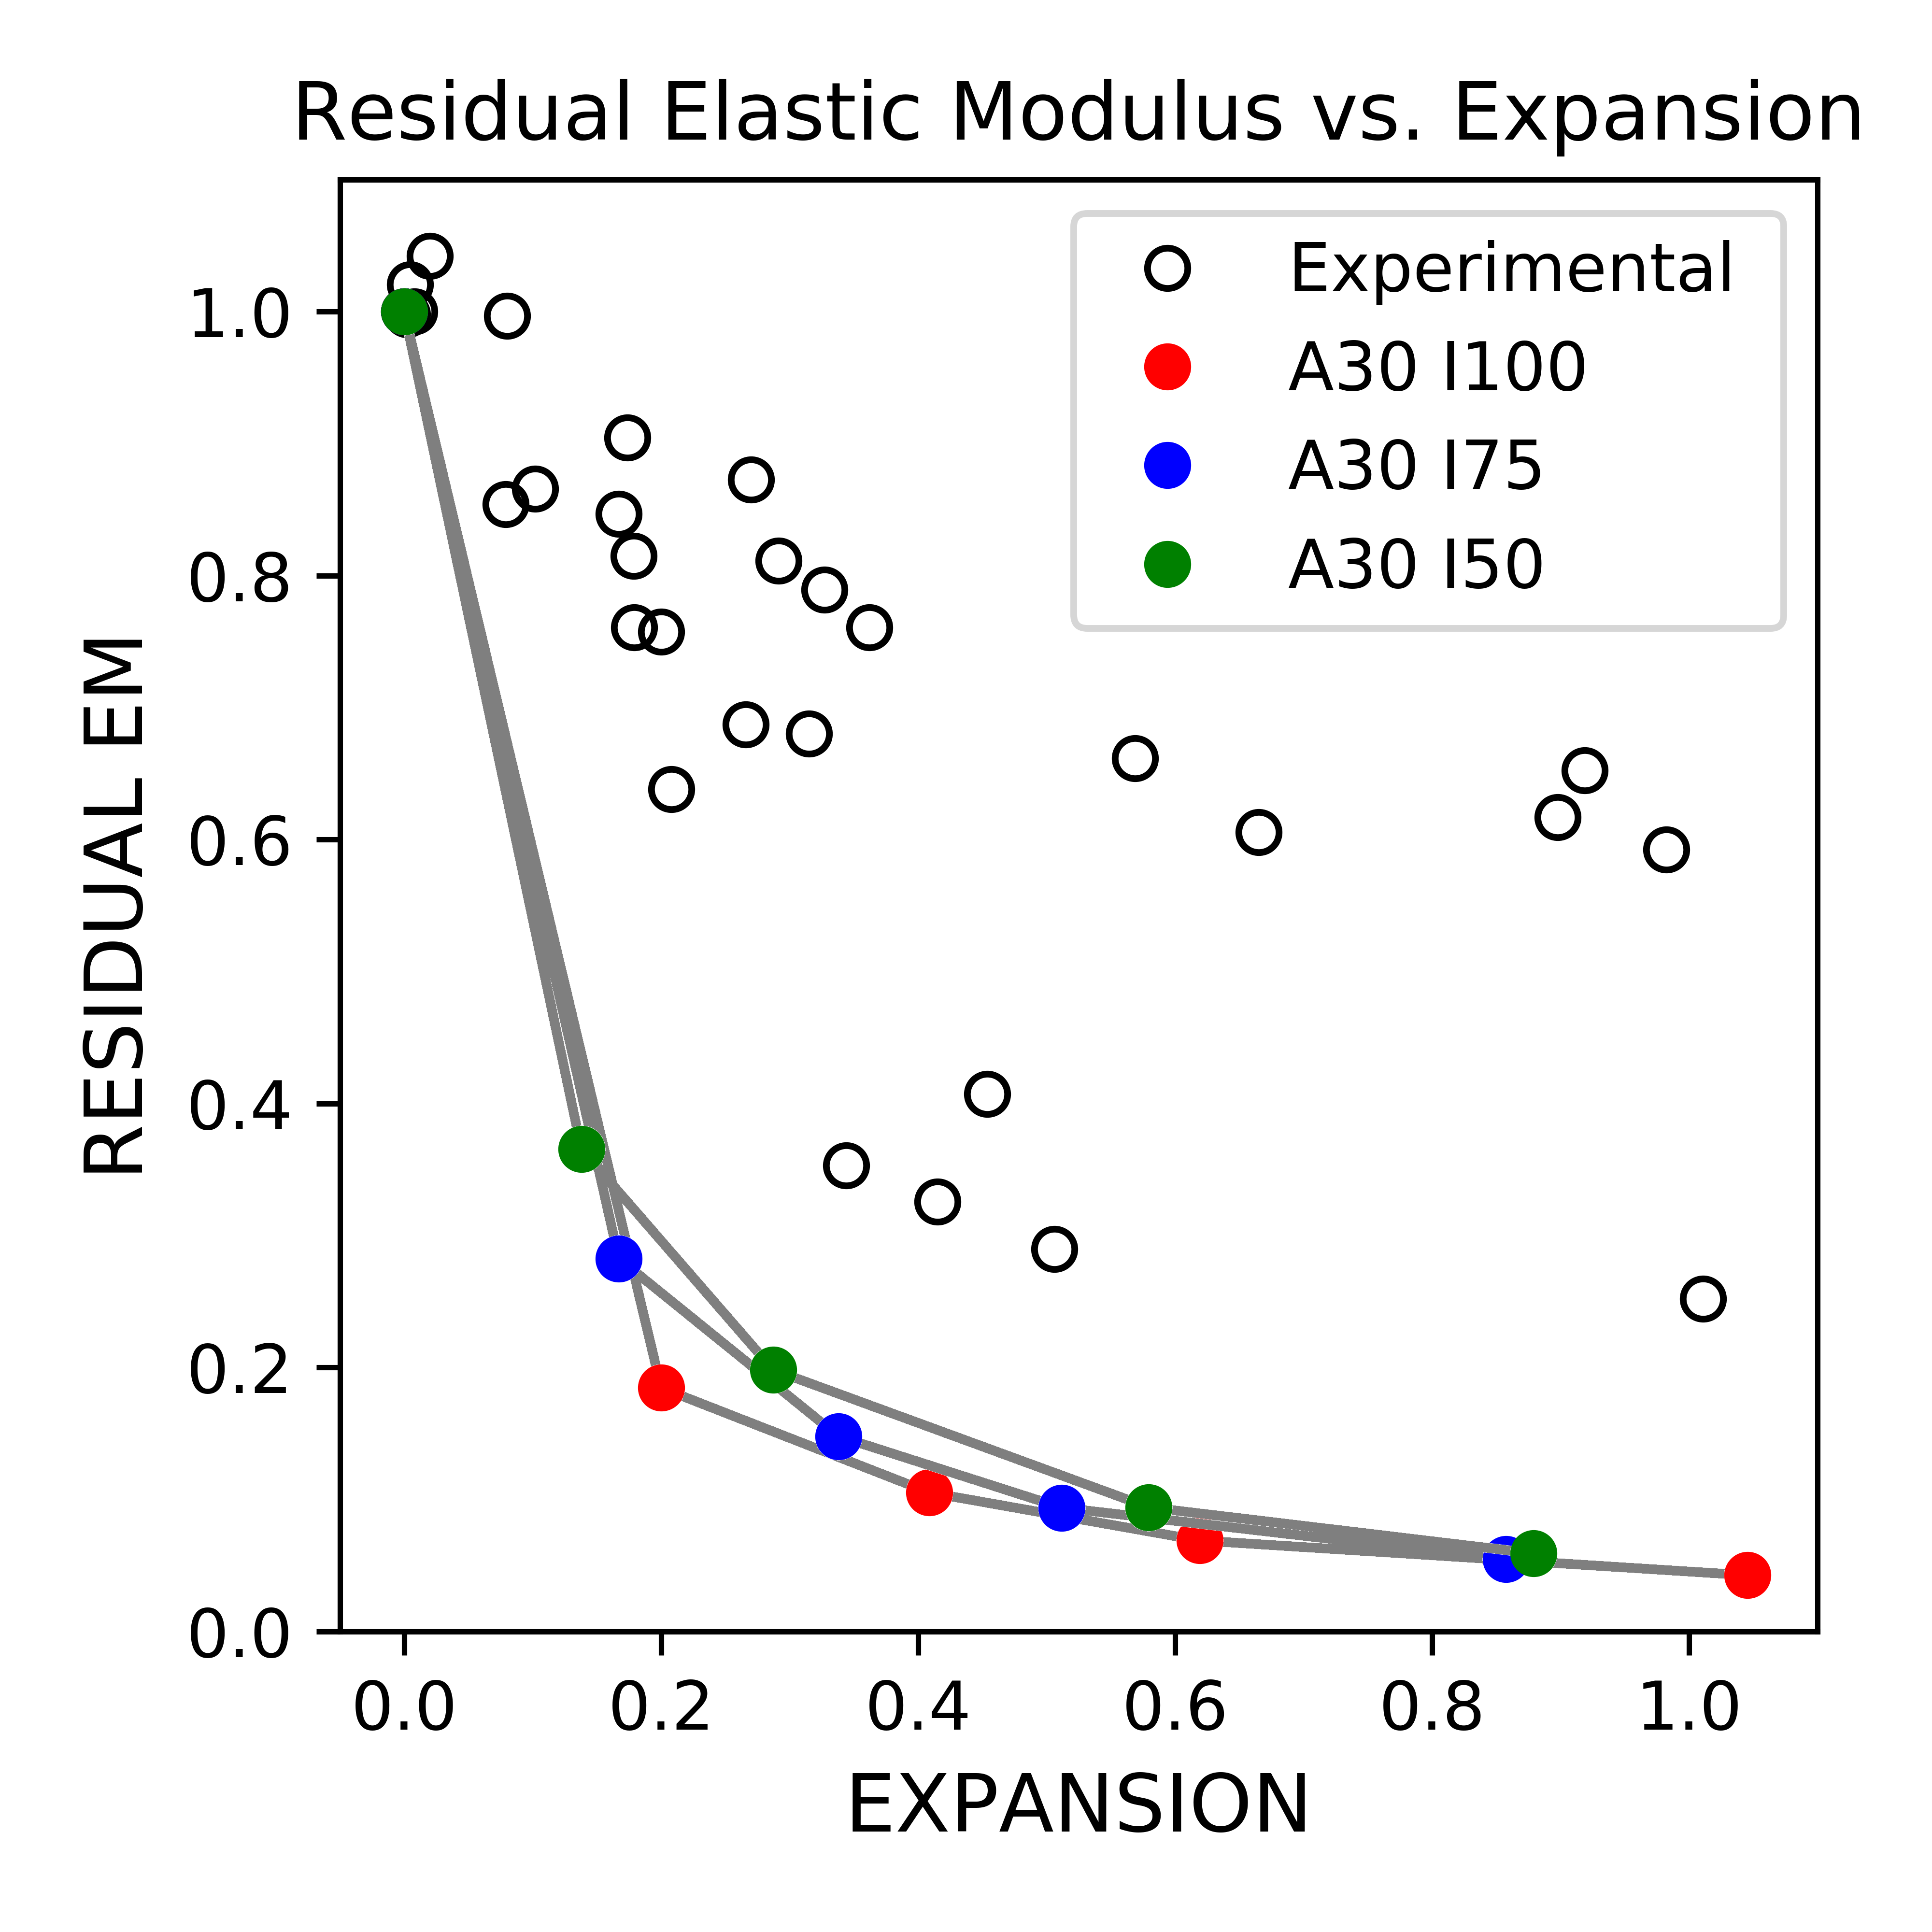
\includegraphics[width=.8\linewidth]{Files/CS_plot/DEFEM3.png}
  \caption{DEF Elastic Modulus Comparing With Experimental Results}
  \label{DEF_X_EM}
\end{figure}

While changing DEF expansion intensified zone does change the cracking pattern signigicantly, the mechanical properties such as compressive strength is not significantly changed.

However, if cross compare the trend in residual compressive strength and residual elastic modulus, shown in Figure \ref{DEF_X} and \ref{DEF_X_EM}, it can be seen that the cases with highest residual compressive strength (which is A30 I100 cases here), are having lowest residual elastic modulus. While the cases with lowest residual compressive strength (which is A30 I50 cases here), are having highest residual elastic modulus.

In later section, further disscussion of the relationship between cracking distribution in DEF expanded concrete model and its residual mechanical properties will also be presented.
